\section*{Experiment 1}

\begin{figure}[H]
\centering
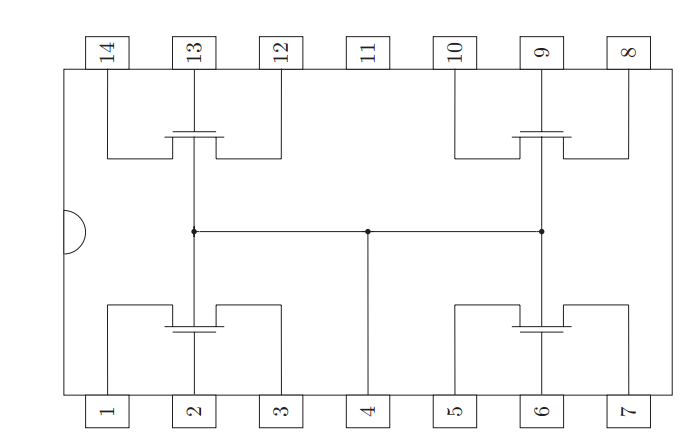
\includegraphics[width=0.65\linewidth]{../Figures/ald1106}
\caption{Picture of the ALD1106 QUAD nMOS transistor array which was used in Experiment 1 to analyze the similarities between nMOS transistors. Using a Quad array is ideal as all transistors are manufactured on the same substrate, optimizing their similarity.}
\label{fig:ald1106}
\end{figure}


In this experiment, we wanted to evaluate how well-matched four nMOS transistors on the same die are. We used the ALD1106 Quad nMOS array, as seen in figure \ref{fig:ald1106}, as all four transistors on this chip are manufactured on the same substrate, which optimizes their similarity. 

We first set the drain voltages of all four transistors to \Vdd and the source voltages to 0, and used the SMU to measure the gate characteristic of each transistor separately. 

\begin{figure}[H]
\centering
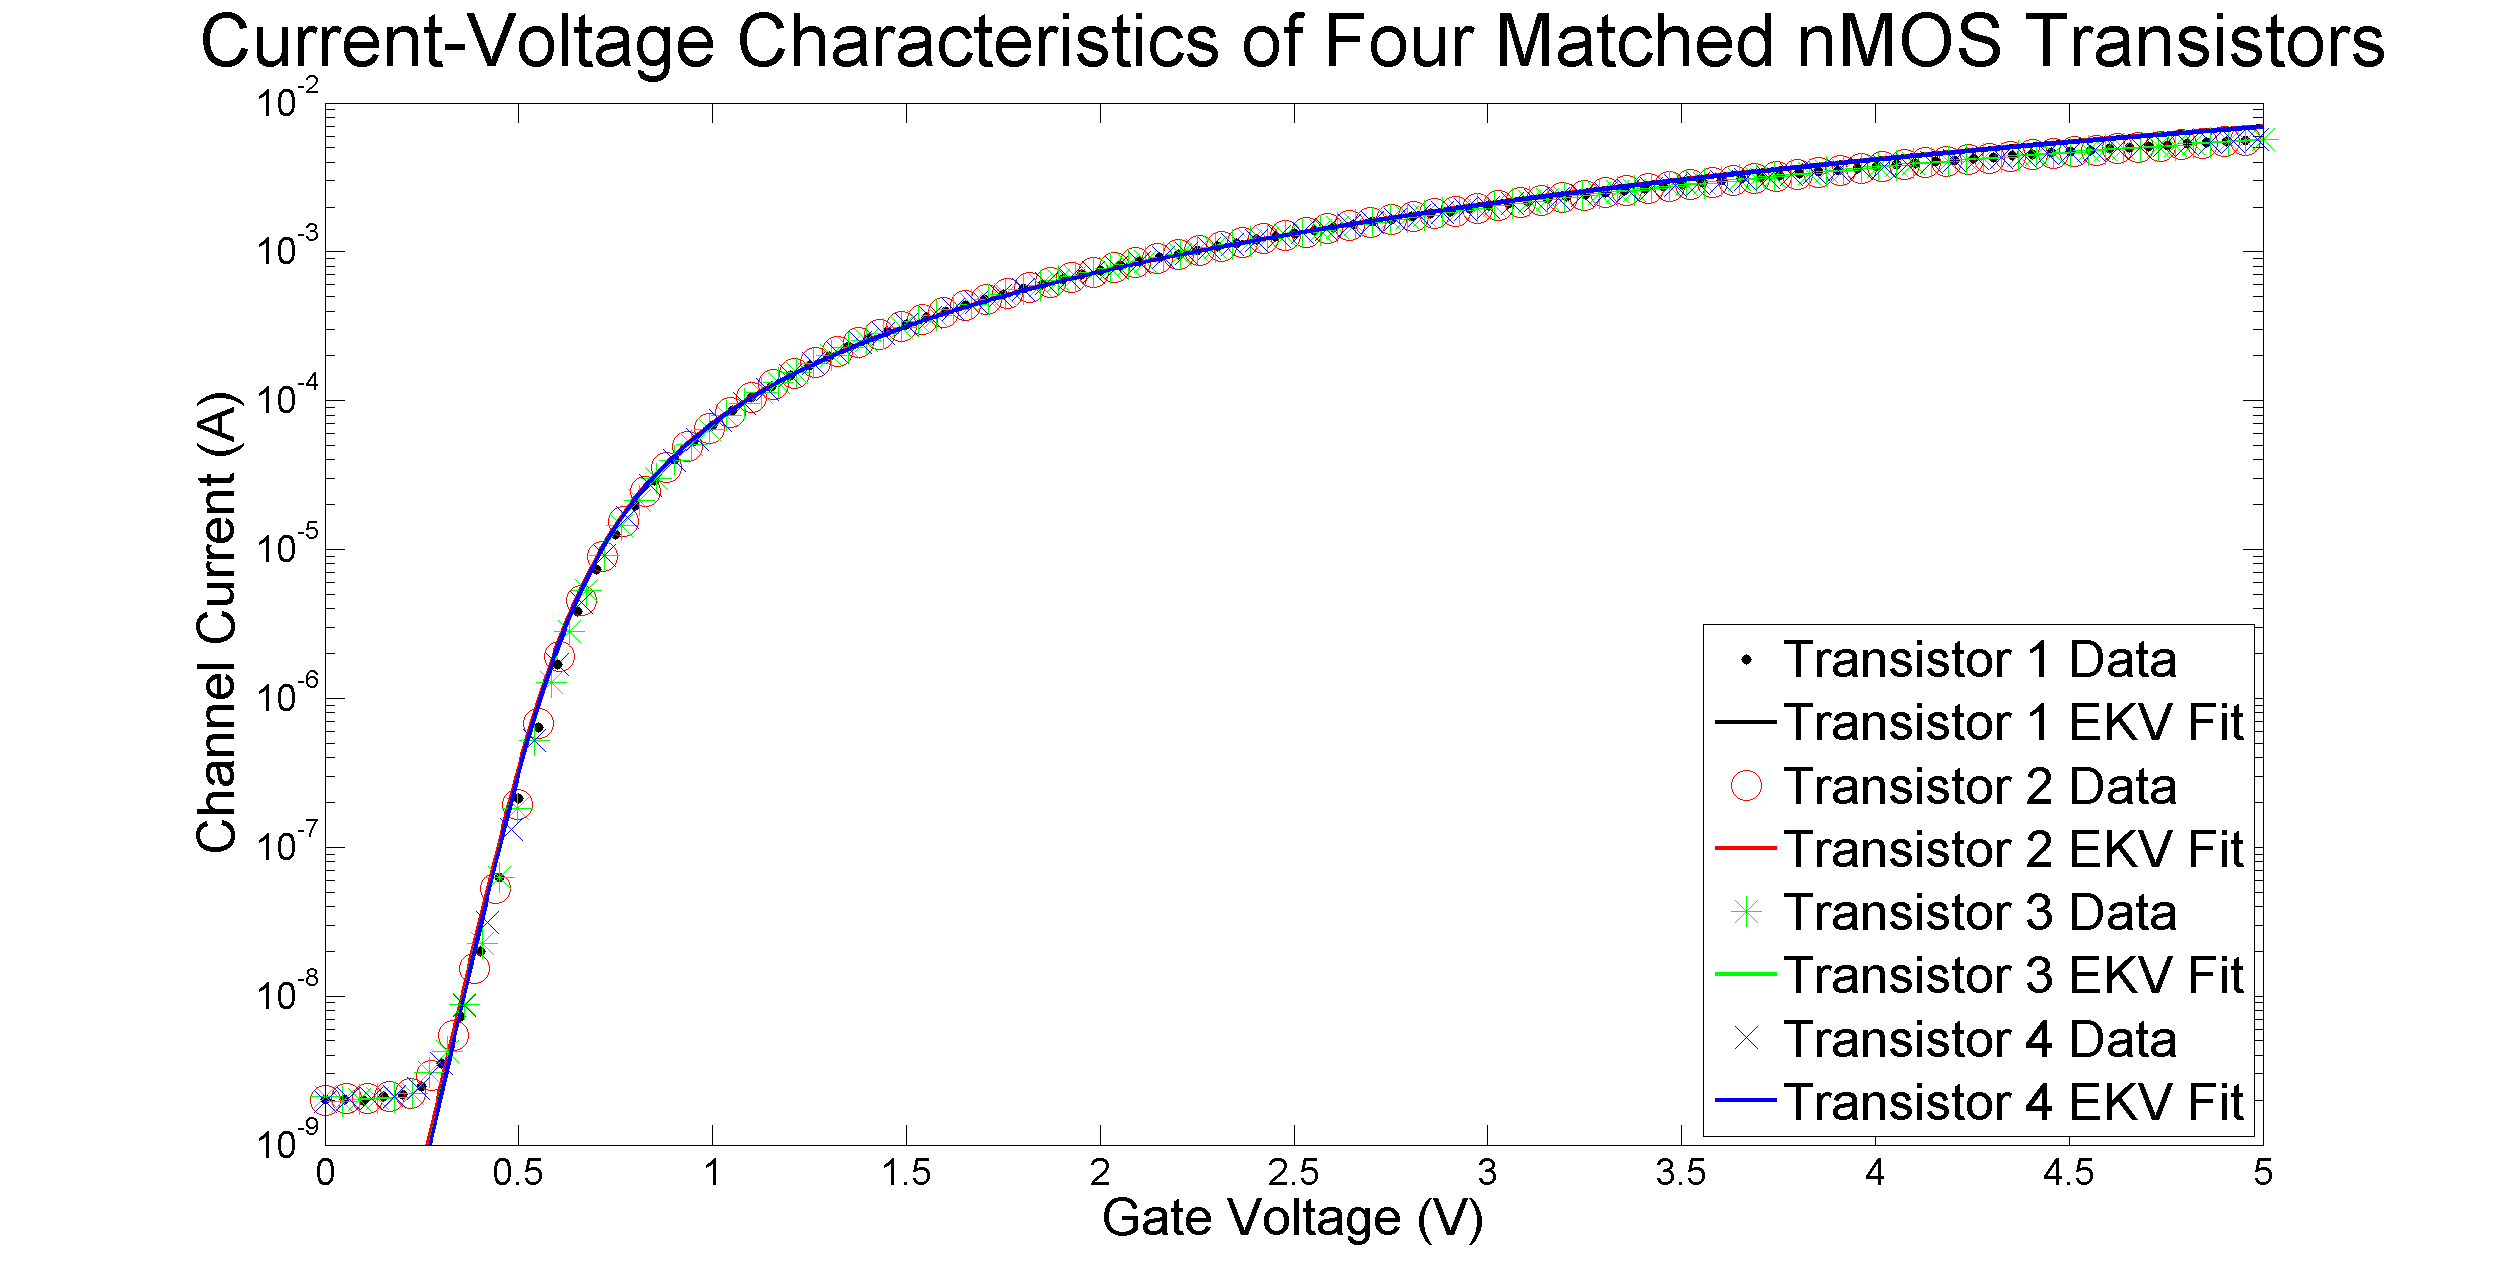
\includegraphics[width=\linewidth]{../Figures/Experiment1Figure1.eps}
\caption{Channel current as a function of gate voltage for four matched nMOS transistors. The theoretical fits generated using the EKV model match the data closely near the middle of the graph, but deviate at small values of gate voltage due to leakage current. The small deviation at large values of gate voltage could be due to \texttt{ekvfit} extracted somewhat incorrect values for $I_s$, which causes the different slopes at large values of gate voltage.}
\label{fig:exp1fig1}
\end{figure}

We then used \texttt{ekvfit.m} to extract balues for $I_s$, $\kappa$, and $V_{T0}$ for each transistor. Table \ref{tb:nmoschar} has the values for these properties for each nMOS transistor:

\begin{table}[h]
\begin{center}
    \begin{tabular}{ l | l | l | l  }
        Transistor & $I_s$ (Amps) & $\kappa$ & $V_{T0}$ (Volts) \\
        \hline
        1 & $1.96 \times 10^{-6}$ & 0.5540  & 0.6912 \\
        2 & $2.02 \times 10^{-6}$ & 0.5521  & 0.6794 \\
        3 & $1.97 \times 10^{-6}$ & 0.5545  & 0.6868 \\
        4 & $1.96 \times 10^{-6}$ & 0.5539  & 0.6892 \\
        \label{tb:nmoschar}
    \end{tabular}
\end{center}
\end{table}

These properties vary little between each transistor, as we expect them to due to the manufacturing process used for the quad chip. The only obvious outlier is the $I_s$ value for transistor 2, which deviates the most from the average $I_s$ value, 1.9775 A. Otherwise we can see that these transistors are very well matched, which should allow for the most accurate current divider ratios in the later part of this lab.

We then used the properties of each transistor along with the EKV model to compare the gate characteristics of all four transistors with theoretical fits, which is shown in figure \ref{fig:exp1fig1}.  The theoretical fits generated using the EKV model match the data closely near the middle of the graph, but deviate at small values of gate voltage due to leakage current. The small deviation at large values of gate voltage could be due to \texttt{ekvfit} extracted somewhat incorrect values for $I_s$, which causes the different slopes at large values of gate voltage.

\begin{figure}[H]
\centering
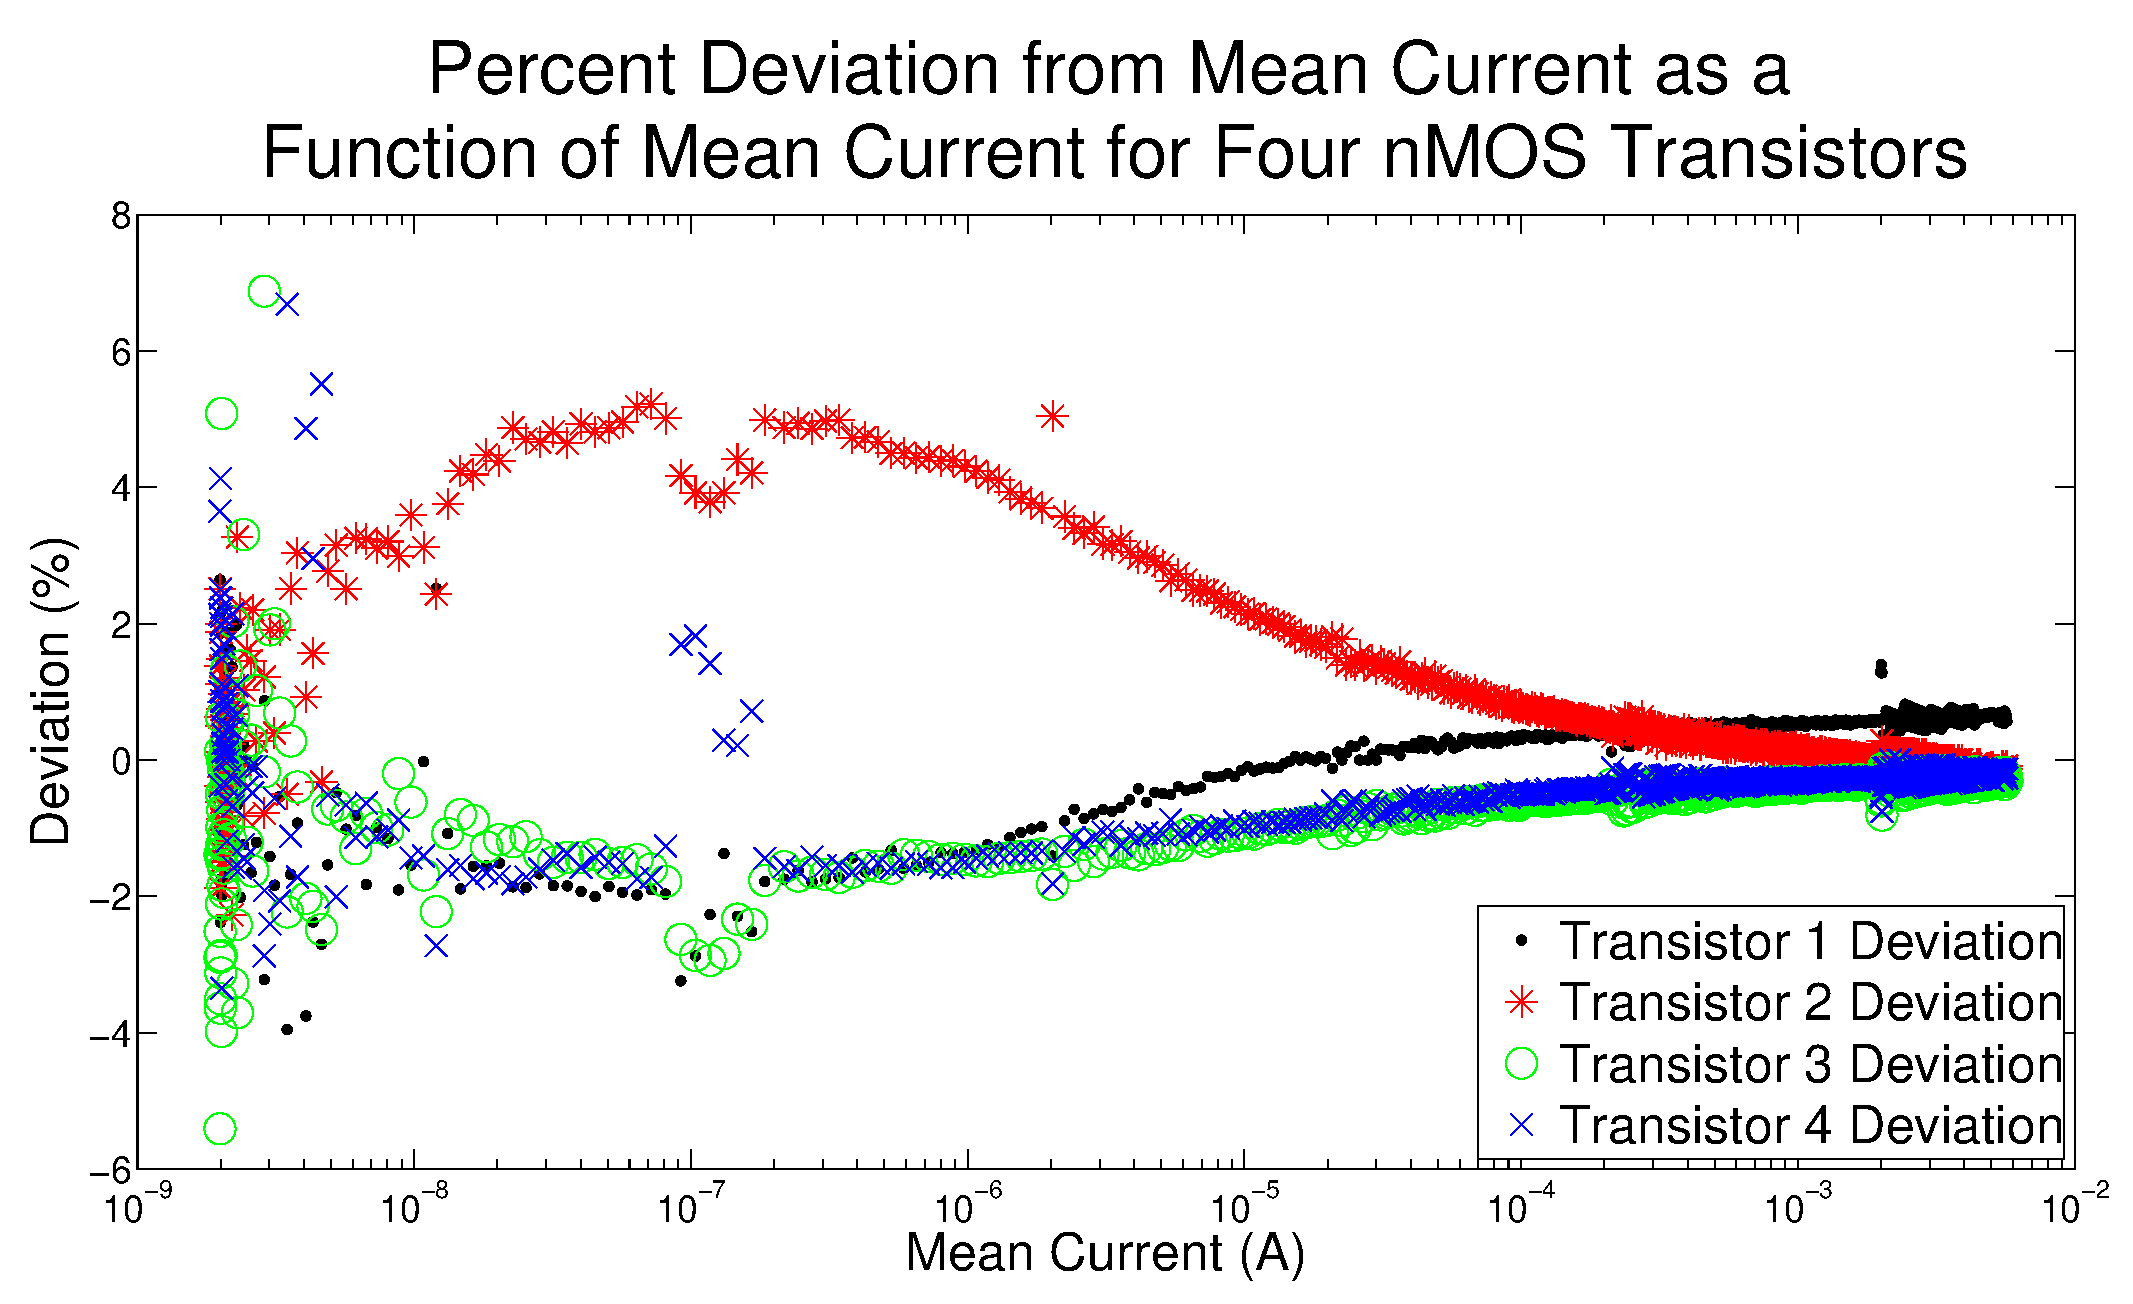
\includegraphics[width=\linewidth]{../Figures/Experiment1Figure2.eps}
\caption{Picture of the ALD1106 QUAD nMOS transistor array which was used in Experiment 1 to analyze the similarities between nMOS transistors. Using a Quad array is ideal as all transistors are manufactured on the same substrate, optimizing their similarity.}
\label{fig:exp1fig2}
\end{figure}

We also looked at all four channel currents as a function of the mean channel current, as seen in figure \ref{fig:exp1fig2}. At very low current values, leakage current and noise caused by the SMU cause the ratio to vary wildly. For currents about a $nA$, however, we saw that the channel currents for transistors 1, 3 and 4 all deviate at about the same percentage relative to the mean current, but the channel current of transistor 2 deviates far more. In fact, we think that the deviation we see in for transistors 1, 3 and 4 is likely due to transistor 2 having a higher strength ratio than the others, causing the higher extracted value for $I_s$, which means a higher channel current, and therefore adjusted the mean channel current causing the other channel currents to deviate below the mean.